% Block diagram of accelerator_alexnet_v2_int16 (ROWS=8, COLS=32).
% Same visual language as img/abstract_arch.png: black outlines, white fill,
% nested boxes, double-headed arrows, sans-serif labels.
% Build:  pdflatex alexnet_v2_arch.tex   (from img/)
\documentclass[tikz,border=4pt]{standalone}
\usepackage[T1]{fontenc}
\usepackage{helvet}
\renewcommand{\familydefault}{\sfdefault}
\usetikzlibrary{arrows.meta,calc}

\begin{document}
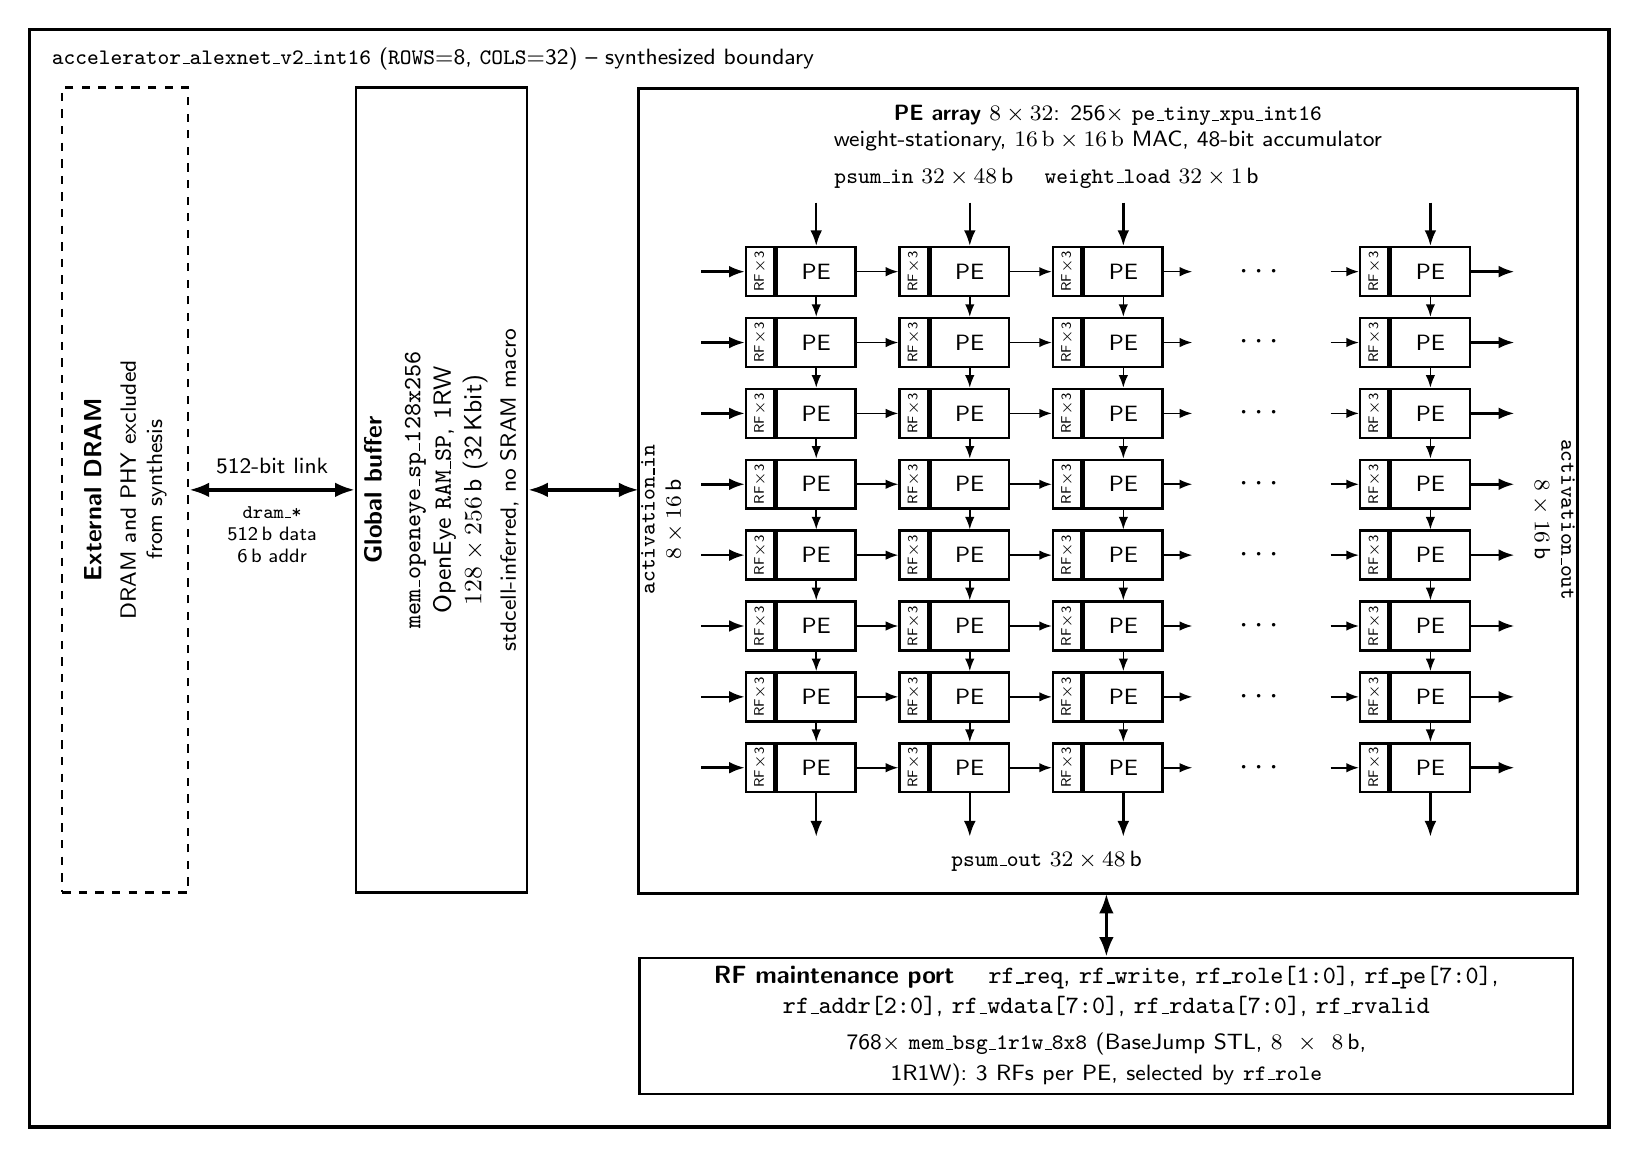
\begin{tikzpicture}[
  font=\small,
  line width=0.9pt,
  blk/.style={draw, fill=white, align=center, inner sep=3pt},
  pe/.style={blk, minimum width=1.0cm, minimum height=0.62cm, font=\footnotesize, inner sep=1pt},
  rf/.style={blk, minimum width=0.36cm, minimum height=0.62cm, inner sep=0pt},
  bus/.style={{Latex[length=2.5mm]}-{Latex[length=2.5mm]}, line width=1.2pt},
  flow/.style={-{Latex[length=1.6mm]}, line width=0.6pt},
  io/.style={-{Latex[length=2mm]}, line width=0.9pt},
  lbl/.style={font=\footnotesize, align=center},
]

% ---------------- PE array ----------------
\def\cpitch{1.95}  % column pitch (cm)
\def\rpitch{0.90}  % row pitch (cm)

% cells: drawn columns 0,1,2 | ... | 31  (index 3 is the ellipsis)
\foreach \r in {0,...,7} {
  \foreach \c in {0,...,4} {
    \pgfmathsetmacro{\cx}{\c*\cpitch}
    \pgfmathsetmacro{\cy}{-\r*\rpitch}
    \ifnum\c=3
      \node[font=\large] at (\cx+0.68,\cy) {$\cdots$};
    \else
      \node[rf, anchor=west] (rf\r\c) at (\cx,\cy) {\rotatebox{90}{\tiny RF$\times$3}};
      \node[pe, anchor=west] (pe\r\c) at (rf\r\c.east) {PE};
    \fi
  }
}

% horizontal activation flow (left -> right)
\foreach \r in {0,...,7} {
  \draw[flow] (pe\r0.east) -- (rf\r1.west);
  \draw[flow] (pe\r1.east) -- (rf\r2.west);
  \draw[flow] (pe\r2.east) -- ++(0.36,0);
  \draw[flow] ($(rf\r4.west)+(-0.36,0)$) -- (rf\r4.west);
}
% vertical partial-sum flow (top -> bottom)
\foreach \r [evaluate=\r as \rn using int(\r+1)] in {0,...,6} {
  \foreach \c in {0,1,2,4} {
    \draw[flow] (pe\r\c.south) -- (pe\rn\c.north);
  }
}

% row I/O: activation_in (left) / activation_out (right)
\foreach \r in {0,...,7} {
  \draw[io] ($(rf\r0.west)+(-0.55,0)$) -- (rf\r0.west);
  \draw[io] (pe\r4.east) -- ($(pe\r4.east)+(0.55,0)$);
}
\node[lbl, rotate=90, anchor=south] at ($(rf00.west)!0.5!(rf70.west)+(-0.65,0)$)
  {\texttt{activation\_in}\\ $8\times16$\,b};
\node[lbl, rotate=-90, anchor=south] at ($(pe04.east)!0.5!(pe74.east)+(0.65,0)$)
  {\texttt{activation\_out}\\ $8\times16$\,b};

% column I/O: psum_in + weight_load (top) / psum_out (bottom)
\foreach \c in {0,1,2,4} {
  \draw[io] ($(pe0\c.north)+(0,0.55)$) -- (pe0\c.north);
  \draw[io] (pe7\c.south) -- ($(pe7\c.south)+(0,-0.55)$);
}
\node[lbl, anchor=south] at ($(pe01.north)!0.5!(pe02.north)+(0,0.6)$)
  {\texttt{psum\_in} $32\times48$\,b \quad \texttt{weight\_load} $32\times1$\,b};
\node[lbl, anchor=north] at ($(pe71.south)!0.5!(pe72.south)+(0,-0.6)$)
  {\texttt{psum\_out} $32\times48$\,b};

% array frame + title
\coordinate (aSW) at ($(rf70.west)+(-1.35,-1.6)$);
\coordinate (aNE) at ($(pe04.east)+(1.35,0)$);
\coordinate (aNE) at ($(aNE|-pe04.north)+(0,2.0)$);
\draw[line width=1.1pt] (aSW) rectangle (aNE);
\node[anchor=north, lbl] at ($(aNE)!0.5!(aNE-|aSW)+(0,-0.08)$)
  {\textbf{PE array $8\times32$}: 256$\times$ \texttt{pe\_tiny\_xpu\_int16}\\
   weight-stationary, $16\,\mathrm{b}\times16\,\mathrm{b}$ MAC, 48-bit accumulator};

% ---------------- RF maintenance port (below the array) ----------------
\path let \p1=(aSW), \p2=(aNE) in
  node[blk, anchor=north west, text width={\x2-\x1-8pt}, minimum height=0.9cm]
  (mport) at ($(aSW)+(0,-0.8)$)
  {\textbf{RF maintenance port} \quad
   \texttt{rf\_req}, \texttt{rf\_write}, \texttt{rf\_role[1:0]}, \texttt{rf\_pe[7:0]},
   \texttt{rf\_addr[2:0]}, \texttt{rf\_wdata[7:0]}, \texttt{rf\_rdata[7:0]}, \texttt{rf\_rvalid}\\[2pt]
   \footnotesize 768$\times$ \texttt{mem\_bsg\_1r1w\_8x8} (BaseJump STL, $8\times8$\,b, 1R1W):
   3 RFs per PE, selected by \texttt{rf\_role}};
\draw[bus] (mport.north) -- (mport.north|-aSW);

% ---------------- Memories on the left ----------------
\path let \p1=(aSW), \p2=(aNE) in
  node[blk, minimum width=1.6cm, minimum height={\y2-\y1}, anchor=south east]
  (gbuf) at ($(aSW)+(-1.4,0)$)
  {\rotatebox{90}{\parbox{7.5cm}{\centering
     \textbf{Global buffer}\\[3pt]
     \texttt{mem\_openeye\_sp\_128x256}\\
     OpenEye \texttt{RAM\_SP}, 1RW\\
     $128\times256$\,b (32\,Kbit)\\[3pt]
     \footnotesize stdcell-inferred, no SRAM macro}}};
\draw[bus] (gbuf.east) -- (gbuf.east-|aSW);

\path let \p1=(aSW), \p2=(aNE) in
  node[blk, dashed, minimum width=1.6cm, minimum height={\y2-\y1}, anchor=south east]
  (dram) at ($(gbuf.south west)+(-2.1,0)$)
  {\rotatebox{90}{\parbox{7.5cm}{\centering
     \textbf{External DRAM}\\[3pt]
     \footnotesize DRAM and PHY excluded\\ from synthesis}}};
\draw[bus] (dram.east) -- (gbuf.west)
  node[midway, above, lbl, yshift=2pt] {512-bit link}
  node[midway, below, lbl, yshift=-2pt, font=\scriptsize]
    {\texttt{dram\_*}\\ 512\,b data\\ 6\,b addr};

% ---------------- Outer frame ----------------
\coordinate (oSW) at ($(dram.south west|-mport.south)+(-0.4,-0.4)$);
\coordinate (oNE) at ($(aNE)+(0.4,0.75)$);
\draw[line width=1.3pt] (oSW) rectangle (oNE);
\node[anchor=north west, lbl] at ($(oSW|-oNE)+(0.15,-0.1)$)
  {\texttt{accelerator\_alexnet\_v2\_int16} (\texttt{ROWS}=8, \texttt{COLS}=32) -- synthesized boundary};

\end{tikzpicture}
\end{document}
